\documentclass[11pt,a4paper]{article}

\usepackage[utf8]{inputenc}
\usepackage[T1]{fontenc}
\usepackage{lmodern}
\usepackage{amsmath,amssymb,mathtools}
\usepackage{graphicx}
\usepackage{booktabs}
\usepackage[margin=1in]{geometry}
\usepackage{natbib}
\usepackage{setspace}
\usepackage{caption}
\usepackage{float}
\usepackage[expansion=false]{microtype}
\usepackage[colorlinks=true,linkcolor=blue,citecolor=blue,urlcolor=blue]{hyperref}
\usepackage[nameinlink,noabbrev]{cleveref}

\graphicspath{{./figures/}}
\onehalfspacing
\setlength{\parskip}{0.35em}

\newcommand{\E}{\mathbb{E}}
\newcommand{\R}{\mathbb{R}}

\title{A corrected-drift Merton benchmark:\\
finite differences, value networks, and a terminal-loss BSDE\\
on three years of Apple prices}

\author{
Arnav Yadav\\
{\small VIT Bhopal University}\\
{\small \href{mailto:arnav.24bai10392@vitbhopal.ac.in}{\texttt{arnav.24bai10392@vitbhopal.ac.in}}}
\and
Somya Patel\\
{\small VIT Bhopal University}\\
{\small \href{mailto:somya.24bsa10058@vitbhopal.ac.in}{\texttt{somya.24bsa10058@vitbhopal.ac.in}}}
}

\date{\today}

\begin{document}
\maketitle

\begin{abstract}
We compare a log-wealth finite-difference grid, a power-scaled value network, a CRRA-shaped value network, and a forward deep BSDE on one Merton problem whose equity coefficients are computed from Apple adjusted closes. The sample is 23~May~2023 through 22~May~2026, the last session in a window opened on 23~May~2023 and closed on 23~May~2026. From 752 log returns the annualized mean log return is $m=0.201649$ and the GBM volatility is $\sigma=0.256573$. The drift in $\mathrm dS/S$ is $\mu=m+\sigma^2/2=0.234564$, not $m$. With $r=0.0368$, $\gamma=5$, and no consumption, the Merton weight is $\pi^{\star}=0.600837$.

On a shared mesh of $10^{4}$ points the $500\times 252$ grid has policy mean absolute error $2.52\times 10^{-4}$. Five seeds of a power-scaled value network, in which a free function $g(t,\log w)$ multiplies the CRRA profile, have policy mean absolute error $1.62\times 10^{-3}$ (sample standard deviation $5.8\times 10^{-4}$) and value mean absolute error $7.09\times 10^{-4}$. The stricter ansatz $g=g(t)$ only forces the weight to equal $\pi^{\star}$ up to roundoff; its value error averages $4.64\times 10^{-4}$. Five seeds of the forward deep BSDE have policy mean absolute error $0.0215$ (standard deviation $0.0072$) and match $V(0,1)$ to about $5\times 10^{-5}$ in $|Y_0-V(0,1)|$. Traded certainty equivalents on $20{,}000$ common paths stay within $10^{-4}$ of the closed-form value $1.10105$ for every one-dimensional method. An Ornstein--Uhlenbeck factor correlated with the stock moves the grid weight at $(t,Y)=(0,0)$ from $0.601$ to $0.499$. The power-scaled network tracks that grid to policy error $0.018$; the deep BSDE, to about $0.097$. A cap $\pi\le 0.4$ binds: the grid weight sits $0.201$ away from $\pi^{\star}$, and the network matches the capped grid to $10^{-8}$. Every printed number is taken from the run ledger. The guide is \texttt{run\_one.py}.
\end{abstract}

\noindent\textbf{Keywords:} Merton problem; GBM drift; finite differences; physics-informed neural networks; deep BSDE.

\section{Contribution and claim limits}
\label{sec:claim}

The note is a controlled numerical comparison, not a new existence theorem and not a claim about $d=100$. \citet{merton1969} and \citet{merton1971} supply the control problem. \citet{raissi2019} and \citet{sirignano2018} supply the value-network methods. \citet{e2017} and \citet{han2018} are cited only for the forward scheme whose loss penalizes $Y_T-U(W_T)$. The martingale objective $-\E[Y_0]+\mathrm{Var}(Y_0)$ is a different algorithm and is not trained here.

What the ledger supports is the following. The drift identity is fixed before training. Five seeds are run for each one-dimensional network at a budget fixed in advance. The finite-difference grid recovers $\pi^{\star}$ at the expected rate in the wealth mesh. The CRRA ansatz is labeled as an ansatz. A one-factor opportunity set, in the sense of \citet{kim1996}, is solved on a $(t,Y)$ grid because wealth separates and the correlated factor does not. A leverage cap that binds is scored against that constrained grid rather than against the unconstrained $\pi^{\star}$.

What is not claimed is a high-dimensional solver, a consumption--investment existence result, or that a small policy error for the CRRA ansatz identifies the weight. The risk-free rate is a declared constant. The equity is one name.

\section{Market coefficients}
\label{sec:market}

Let $S_t$ be the adjusted close. Daily log returns on the 753 sessions from 23~May~2023 through 22~May~2026 give $n=752$ increments. With a 252-day year,
\begin{align}
m &= 252\cdot \frac{1}{n}\sum_{i=1}^{n}\log\frac{S_{i}}{S_{i-1}} = 0.20164940530246397,\\
\sigma &= \sqrt{252}\; s_{n-1}(\log S_{i}/S_{i-1}) = 0.2565727586666484.
\end{align}
If $\mathrm dS/S=\mu\,\mathrm dt+\sigma\,\mathrm dB$, then $\E[\log(S_{t+\Delta}/S_t)]=(\mu-\sigma^2/2)\Delta t$, so the drift that enters the wealth equation is
\begin{equation}
\mu = m+\sigma^2/2 = 0.23456419554737107.
\end{equation}
A fresh \texttt{yfinance} download of the same window reproduced $m$ and $\sigma$ within $10^{-7}$. The frozen file keeps the stored pair. The constant $r=0.0368$ is not a Treasury-bill average. Relative risk aversion is $\gamma=5$, the horizon is $T=1$, and initial wealth is $W_0=1$. There is no consumption in the one-dimensional block or in the factor block.

\begin{table}[H]
\centering
\caption{Quantities that are not interchangeable. $m$ is the mean log return. $\mu$ is the GBM drift.}
\label{tab:market}
\begin{tabular}{lr}
\toprule
Quantity & Value \\
\midrule
$m$ & 0.201649405302464 \\
$\sigma^2/2$ & 0.032914790244907 \\
$\mu=m+\sigma^2/2$ & 0.234564195547371 \\
$\sigma$ & 0.256572758666648 \\
$r$ & 0.0368 \\
$\gamma$ & 5 \\
$\pi^{\star}=(\mu-r)/(\gamma\sigma^2)$ & 0.600836870221195 \\
$V(0,1)$ & $-0.170138511234813$ \\
\bottomrule
\end{tabular}
\end{table}

Putting $m$ in the drift slot changes the weight from $0.600837$ to $0.500837$. Checkpoints trained on that substitution are not rescored in this paper.

\section{The control problem}
\label{sec:control}

Wealth in the risky asset and the constant money-market account obeys
\begin{equation}
\mathrm dW_t = W_t\big(r+\pi_t(\mu-r)\big)\,\mathrm dt + W_t\pi_t\sigma\,\mathrm dB_t,
\end{equation}
and the investor maximizes $\E[U(W_T)]$ with
\begin{equation}
U(w)=\frac{w^{1-\gamma}}{1-\gamma}, \qquad \gamma>1.
\end{equation}
The value $V(t,w)$ solves the Hamilton--Jacobi--Bellman equation of \citet{merton1969},
\begin{equation}
V_t + \sup_{\pi}\Big\{w\big(r+\pi(\mu-r)\big)V_w + \tfrac12 \pi^2\sigma^2 w^2 V_{ww}\Big\} = 0,
\end{equation}
with $V(T,w)=U(w)$. The maximizer and the value are
\begin{align}
\pi^{\star} &= \frac{\mu-r}{\gamma\sigma^2},\\
V(t,w) &= \mathrm e^{A(T-t)}\frac{w^{1-\gamma}}{1-\gamma},\\
A &= (1-\gamma)\left(r+\frac{(\mu-r)^2}{2\gamma\sigma^2}\right).
\end{align}
On the frozen coefficients, $\pi^{\star}=0.600836870221195$ and $V(0,1)=-0.170138511234813$.

\section{Numerical methods}
\label{sec:methods}

\subsection{Finite differences}

The grid is written in log-wealth $x=\log w$ on $x\in[-2.5,4.5]$, with an implicit ($\theta=1$) upwind scheme. The candidate weight at each node is the first-order condition
\begin{equation}
\pi = -\frac{(\mu-r)V_x}{\sigma^2(V_{xx}-V_x)},
\end{equation}
clipped to $[-1,5]$ in the unconstrained runs and to $[0,0.4]$ in the constrained runs. Non-finite first-order conditions are replaced by $0$, not by $\pi^{\star}$. The release grid is $N_x=500$, $N_t=252$.

\subsection{Collocation and the terminal condition}

Both value networks draw a fresh Latin hypercube at every Adam step. Interior points use two dimensions: time uniform on $[0,T]$ and wealth uniform on $[0.5,2]$, jointly. The one-dimensional budget is $25{,}000$ interior points. Terminal points use a one-dimensional hypercube of $8{,}000$ wealth samples on the same interval, with time pinned at $T$ and target $U(w)$. The sampler seed is a function of the run seed and the epoch, so a repeated command with the same seed replays the same minibatches on the same device class.

The unstructured network of \citet{raissi2019} is given a power head so that the output lives on the scale of $U$. Five $\tanh$ layers of width 128 map $(\log w, t)$ to a scalar $g$, and
\begin{equation}
V(t,w)=\mathrm e^{g(t,\log w)}\frac{w^{1-\gamma}}{1-\gamma}.
\end{equation}
Because $g$ may depend on wealth, $V_w/(w V_{ww})$ is not identically $1/\gamma$. The network does not output $\pi$. After training, the weight is the first-order condition on the automatic derivatives. The loss is the mean square HJB residual, plus ten times the relative terminal mismatch, plus $0.1$ times the squared positive part of $V_{ww}$ and of $-V_w$. The residual uses the reduced unconstrained Hamiltonian unless the run is the capped problem, in which case the Hamiltonian is evaluated at $\pi$ projected onto $[0,0.4]$. A raw network with no power head was not used: on this utility its target ranges over orders of magnitude inside $[0.5,2]$, and the head removes that scale without inserting $\pi^{\star}$.

\subsection{The CRRA ansatz}

The shaped network is
\begin{equation}
V(t,w)=\mathrm e^{g_\theta(t)}\frac{w^{1-\gamma}}{1-\gamma}.
\end{equation}
For any $g_\theta$, $V_w/(w V_{ww})=1/\gamma$, so the induced weight equals $\pi^{\star}$ up to roundoff whenever $\mu$, $r$, $\sigma$, and $\gamma$ are the training coefficients. A policy error of size $10^{-8}$ on this model is a derivative check. The trained object is $g_\theta$, and the reported error is the error in $V$.

\subsection{Forward deep BSDE}

Following the forward discretization of \citet{han2018} and \citet{e2017}, a scalar $Y_0$ and a network $Z$ are stepped along the controlled wealth. There is no running consumption, and under a Markov control the value along the path is a martingale when the HJB residual vanishes, so the increment is
\begin{equation}
Y \leftarrow Y + Z(t,W)\,\Delta B
\end{equation}
with $Z$ evaluated at the wealth observed before that Brownian increment is applied. The policy network enters only through $W$. Its range is $(-2,2)$ via $2\tanh$. The loss on each batch of $1{,}024$ paths and $64$ steps is
\begin{equation}
\E\big[(Y_T-U(W_T))^2\big] - \E[U(W_T)].
\end{equation}
The mean-square term trains $(Y_0,Z)$. The utility term is what moves the policy: a pure terminal match can be achieved for a poor control if $Z$ is flexible. $Y_0$ is initialized at $U(W_0)$, not at the closed form. This scheme is not the martingale objective that assigns $Y_T=U(W_T)$ and scores $-\E[Y_0]+\mathrm{Var}(Y_0)$.

\subsection{Protocol}

Adam uses learning rate $10^{-3}$. One-dimensional networks run $2{,}000$ epochs. The best-loss weights are kept. Seeds are $\{0,1,2,3,4\}$ for the vanilla network, the ansatz, and the deep BSDE. The mesh used for every one-dimensional table has $10^{4}$ points, seed $12345$, wealth log-uniform on $[0.5,2]$, and time uniform on $[0,1)$. Traded utility uses $20{,}000$ paths, $252$ steps, and seed $7$, the same paths for every method. Certainty equivalent wealth is the $w$ with $U(w)=\E[U(W_T)]$. Device was CUDA. Floats will move on CPU; the seeds and the pass band on the grid will not.

\section{One-dimensional results}
\label{sec:results1d}

\subsection{The grid}

Experiment E1 is the $500\times 252$ solve on $\mu$. Policy mean absolute error on the mesh is $2.5217\times 10^{-4}$. The error is almost constant across the mesh (the root mean square matches the mean absolute error), which is what a constant-weight solution looks like when the grid's $\pi$ is a single biased number. The value at the node nearest $(t,W)=(0,1)$ is $-0.169453$, against $-0.170139$. Mesh value mean absolute error is $4.398\times 10^{-3}$. On the common paths the closed-form weight and the grid weight both have certainty equivalent $1.10105$ to five decimals (mean utility $-0.170103$).

\begin{table}[H]
\centering
\caption{Finite-difference refinement (E2). Policy error tracks $N_x$. Extra time steps do not move $\pi$.}
\label{tab:fdm}
\begin{tabular}{rrrr}
\toprule
$N_x$ & $N_t$ & policy MAE & value MAE \\
\midrule
128 & 64  & $3.878\times 10^{-3}$ & $1.620\times 10^{-2}$ \\
128 & 128 & $3.878\times 10^{-3}$ & $1.641\times 10^{-2}$ \\
128 & 252 & $3.878\times 10^{-3}$ & $1.652\times 10^{-2}$ \\
256 & 64  & $9.649\times 10^{-4}$ & $8.223\times 10^{-3}$ \\
256 & 128 & $9.649\times 10^{-4}$ & $8.413\times 10^{-3}$ \\
256 & 252 & $9.649\times 10^{-4}$ & $8.506\times 10^{-3}$ \\
500 & 64  & $2.522\times 10^{-4}$ & $4.134\times 10^{-3}$ \\
500 & 128 & $2.522\times 10^{-4}$ & $4.311\times 10^{-3}$ \\
500 & 252 & $2.522\times 10^{-4}$ & $4.398\times 10^{-3}$ \\
\bottomrule
\end{tabular}
\end{table}

Quadrupling $N_x$ from 128 to 500 cuts the policy error by about fifteen, close to a second-order spatial gain on this smooth solution. Value error on the random mesh does not fall when $N_t$ rises. The policy, which is what is traded, is already settled by the spatial grid.

\begin{figure}[H]
\centering
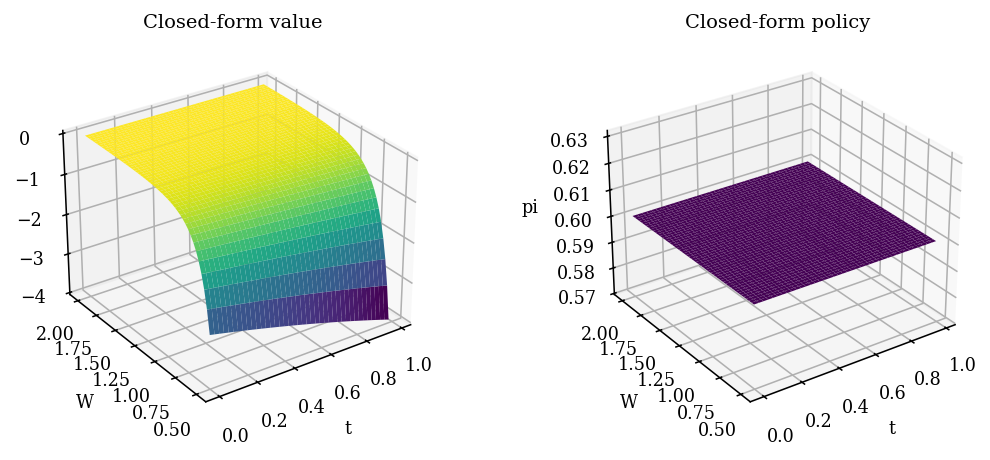
\includegraphics[width=0.92\textwidth]{surface_closed.png}
\caption{Closed-form value and the constant weight $\pi^{\star}$ on $(t,W)\in[0,0.98]\times[0.5,2]$.}
\label{fig:closed}
\end{figure}

\begin{figure}[H]
\centering
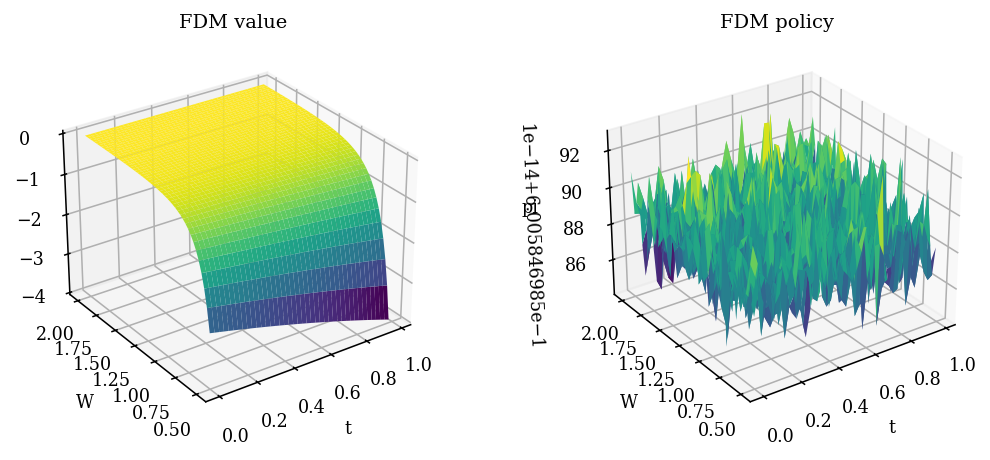
\includegraphics[width=0.92\textwidth]{surface_fdm.png}
\caption{E1 finite-difference value and policy on the same window. The policy surface is flat at $\pi^{\star}$ up to the $2.5\times 10^{-4}$ bias in \Cref{tab:fdm}.}
\label{fig:fdm}
\end{figure}

\subsection{Neighbour grids}

Experiment E6 reruns the $256\times 128$ grid at $\gamma\in\{3,7\}$ and at $\sigma$ scaled by $0.8$ and $1.2$, still on the corrected drift formula. Policy mean absolute error stays between $3.4\times 10^{-4}$ and $1.7\times 10^{-3}$. The grid is not tuned to the single Apple point $(\gamma,\sigma)=(5,0.256573)$.

\begin{table}[H]
\centering
\caption{E6. Each row is a new solve. $\pi^{\star}$ changes with the row. The error is against that row's closed form.}
\label{tab:sens}
\begin{tabular}{rrrr}
\toprule
$\gamma$ & $\sigma$ & $\pi^{\star}$ & policy MAE \\
\midrule
3 & 0.256573 & 1.001395 & $3.353\times 10^{-4}$ \\
7 & 0.256573 & 0.429169 & $1.659\times 10^{-3}$ \\
5 & 0.205258 & 0.938808 & $1.508\times 10^{-3}$ \\
5 & 0.307887 & 0.417248 & $6.701\times 10^{-4}$ \\
\bottomrule
\end{tabular}
\end{table}

\subsection{Five seeds of the ansatz}

E4 trains the shaped value network for $2{,}000$ epochs. Policy mean absolute error is between $3.18\times 10^{-8}$ and $3.26\times 10^{-8}$ on every seed. That number is not a portfolio result. Value mean absolute error on the mesh has mean $4.64\times 10^{-4}$ and sample standard deviation $1.81\times 10^{-4}$ across the five seeds (the five errors are $4.61$, $3.02$, $6.42$, $6.49$, and $2.66$ times $10^{-4}$). Traded certainty equivalents match the closed-form paths at $1.10105$, as they must once the weight is $\pi^{\star}$.

\subsection{Power-scaled value network}

E3 trains $V=\mathrm e^{g(t,\log w)}w^{1-\gamma}/(1-\gamma)$ for $2{,}000$ epochs, five seeds, $25{,}000$ collocation points and $8{,}000$ terminal points. Policy mean absolute errors are $1.81\times 10^{-3}$, $2.41\times 10^{-3}$, $1.46\times 10^{-3}$, $8.14\times 10^{-4}$, and $1.60\times 10^{-3}$. The mean is $1.62\times 10^{-3}$ and the sample standard deviation is $5.79\times 10^{-4}$. Value mean absolute errors average $7.09\times 10^{-4}$ with standard deviation $1.60\times 10^{-4}$. That is slightly larger than the time-only ansatz. The weight is no longer an identity, and it is still within a few times the grid's $2.52\times 10^{-4}$. Traded certainty equivalents average $1.1010493$, against $1.1010499$ for the closed-form weight on the same paths.

\subsection{Forward deep BSDE}

E5 trains five seeds for $2{,}000$ epochs on $1{,}024$ paths and $64$ steps. Policy mean absolute errors are $0.03019$, $0.01840$, $0.02672$, $0.01184$, and $0.02021$. The mean is $0.02147$ and the sample standard deviation is $0.00720$. The absolute gap $|Y_0-V(0,1)|$ averages $4.85\times 10^{-5}$ (standard deviation $3.83\times 10^{-5}$). Traded certainty equivalents average $1.100984$, about $6.5\times 10^{-5}$ below the closed-form paths. The initial condition of the BSDE is accurate. The portfolio weight on the mesh is less accurate than the grid and less accurate than the power-scaled value network. Both facts are in \Cref{tab:main1d}.

\begin{table}[H]
\centering
\caption{One-dimensional mesh errors, means over seeds. The CRRA policy error is a derivative check. Sample standard deviations are in the reproducibility section. Closed-form certainty equivalent on the common paths: $1.101050$. Traded: grid $1.101050$, ansatz $1.101050$, power-scaled $1.101049$, deep BSDE $1.100984$.}
\label{tab:main1d}
{\small
\begin{tabular}{lrrrr}
\toprule
Method & seeds & policy MAE & value MAE & $|Y_0-V(0,1)|$ \\
\midrule
FDM $500\times 252$ & 1 & $2.52\times 10^{-4}$ & $4.40\times 10^{-3}$ & --- \\
CRRA $g(t)$ & 5 & $3.2\times 10^{-8}$ & $4.6\times 10^{-4}$ & --- \\
Power $g(t,\log w)$ & 5 & $1.6\times 10^{-3}$ & $7.1\times 10^{-4}$ & --- \\
Deep BSDE & 5 & $2.1\times 10^{-2}$ & --- & $4.9\times 10^{-5}$ \\
\bottomrule
\end{tabular}
}
\end{table}

\section{A factor in the drift}
\label{sec:factor}

Constant-coefficient CRRA wealth collapses to a one-dimensional PDE, so a second risky asset with constant coefficients would not stress the grid. The extension follows the stochastic opportunity set of \citet{kim1996}. The factor is Ornstein--Uhlenbeck,
\begin{equation}
\mathrm dY_t = -\kappa Y_t\,\mathrm dt + \nu\,\mathrm dB^Y_t,
\end{equation}
with $\kappa=1.2$, $\nu=0.30$, and $\mathrm{Corr}(\mathrm dB,\mathrm dB^Y)=\rho=0.45$. The stock drift is $\mu+\phi Y$ with $\phi=0.20$. Wealth still separates,
\begin{equation}
V(t,w,y)=f(t,y)\frac{w^{1-\gamma}}{1-\gamma},
\end{equation}
but the first-order condition contains a hedge term,
\begin{equation}
\pi^{\star}(t,y)=\frac{\mu+\phi y-r}{\gamma\sigma^2}+\frac{\rho\nu}{\sigma\gamma}\frac{f_y}{f}.
\end{equation}
The function $f$ is not constant in $y$. It is computed on a grid of $81$ factor nodes on $[-1.5,1.5]$ and $200$ time steps, with the policy lagged one time level inside a linear implicit step. Neumann conditions close the ends. The same code with $\phi=0$ and $\rho=0$ reproduces $\mathrm e^{AT}$ with max absolute error $2.52\times 10^{-4}$, which is the check that the factor scheme has not been given a free constant.

The factor PINN learns $g(t,y)$ in $f=\mathrm e^{g}$, with $4{,}096$ Latin-hypercube collocation points and a terminal penalty $g(T,y)=0$. The factor BSDE carries two Brownian increments, evaluates both components of $Z$ before the state is updated, and uses the same terminal-loss-plus-utility objective. E7 is seed 0 and E8 is seed 1, each for $800$ epochs. Both are scored against the factor grid on $4{,}000$ points, not against the constant $\pi^{\star}$.

At the Apple coefficients the factor grid gives $\pi(0,0)=0.49918$ and $V(0,1,0)=-0.16217$, against the constant-opportunity values $0.60084$ and $-0.17014$. The hedge term and the state-dependent drift are visible: the weight is no longer $\pi^{\star}$.

E7 and E8 train the factor network and the two-noise deep BSDE for $800$ epochs. Policy mean absolute error of the power head against the factor grid is $0.01810$ (seed 0) and $0.01861$ (seed 1). Value error is $0.0437$ and $0.0451$. The deep BSDE policy errors are $0.0949$ and $0.0994$. Its $Y_0$ is about $-0.1717$, against the grid value $-0.1622$ at $(W,Y)=(1,0)$, a gap of $9.6\times 10^{-3}$. On this problem the value network follows the grid more closely than the BSDE. \Cref{fig:factor} is the grid policy over $(t,Y)$.

\begin{table}[H]
\centering
\caption{Factor model against the $(t,Y)$ grid. Two seeds, $800$ epochs. $\pi(0,0)$ and $V(0,1,0)$ are grid quantities and do not depend on the seed.}
\label{tab:factor}
\begin{tabular}{lrr}
\toprule
 & seed 0 & seed 1 \\
\midrule
Power-head policy MAE & 0.01810 & 0.01861 \\
Power-head value MAE & 0.04368 & 0.04511 \\
Deep BSDE policy MAE & 0.09488 & 0.09940 \\
$|Y_0-V_{\mathrm{grid}}(0,1,0)|$ & 0.00957 & 0.00954 \\
\bottomrule
\end{tabular}
\end{table}

\section{A cap that binds}
\label{sec:cap}

The unconstrained weight is about $0.60$, so the interval $[0,1]$ does not bind. E9 and E10 use $\pi\in[0,0.4]$. For constant coefficients the constrained optimum is the projection of $\pi^{\star}$ onto that interval, and the grid is still the reference the network is scored against. The vanilla PINN is trained with the Hamiltonian evaluated at the projected control, $2{,}000$ epochs, seeds 0 and 1. A network that reports $\pi^{\star}$ on this problem is wrong.

E9 and E10 are seeds 0 and 1 of that capped solve, $400\times 200$ in the grid and $2{,}000$ epochs in the network. The constrained grid's weight differs from $\pi^{\star}$ by mean absolute error $0.200837$, which is $\pi^{\star}-0.4$ when the cap binds at every mesh point. The power-scaled network, trained with the projected Hamiltonian, matches that grid's weight to $6.0\times 10^{-9}$ on both seeds. Value error against the grid is $4.12\times 10^{-3}$ and $4.15\times 10^{-3}$. The grid value at the node nearest $(0,1)$ is $-0.166096$, above the unconstrained $-0.170139$ (less negative, because the forbidden leverage was valuable). The network did not report the unconstrained weight.

\section{What the pictures are for}
\label{sec:fig}

\begin{figure}[H]
\centering
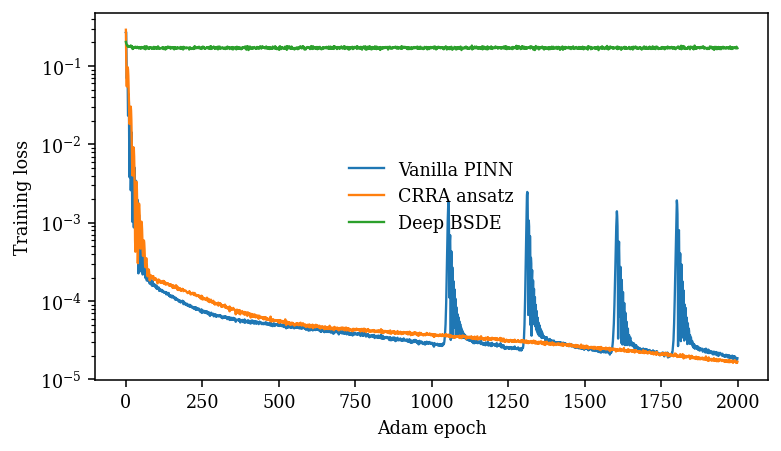
\includegraphics[width=0.86\textwidth]{training_loss.png}
\caption{Training loss at every epoch for seed 0 of the power-scaled network, the CRRA ansatz, and the deep BSDE. The saved weights are the minimizer of the curve, not the last epoch.}
\label{fig:loss}
\end{figure}

\begin{figure}[H]
\centering
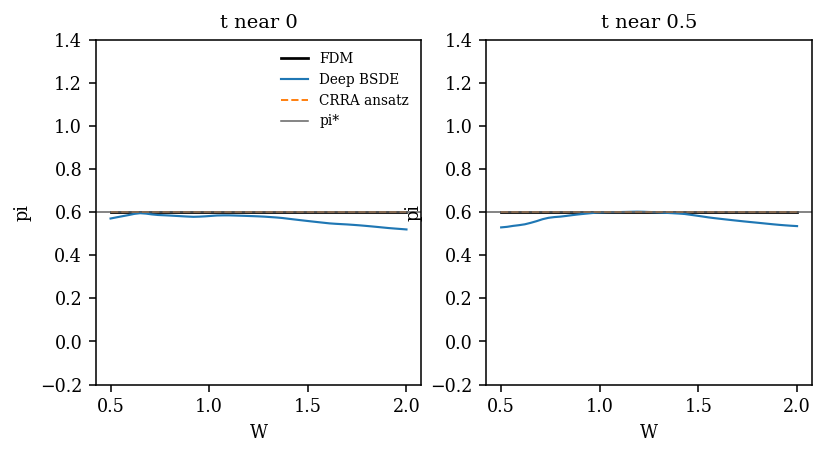
\includegraphics[width=0.92\textwidth]{policy_slices.png}
\caption{Policy against wealth at two times for the grid, the CRRA ansatz, and deep BSDE seed 0. The axis is the scale of $\pi^{\star}$.}
\label{fig:slices}
\end{figure}

\begin{figure}[H]
\centering
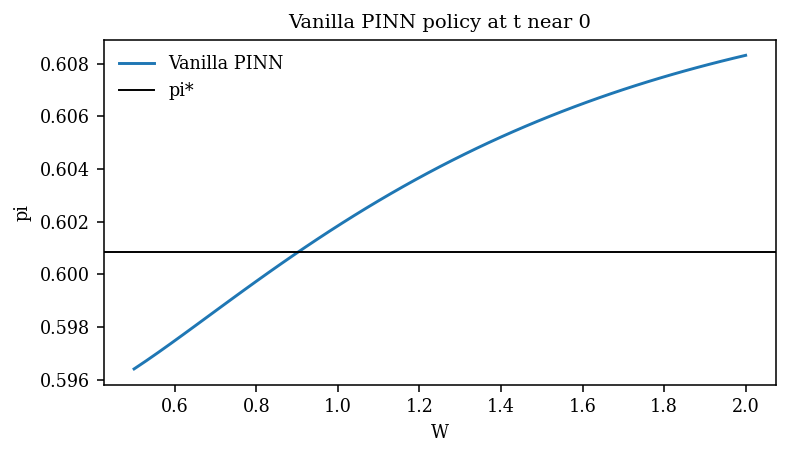
\includegraphics[width=0.72\textwidth]{policy_pinn_slice.png}
\caption{Seed-0 power-scaled policy near $t=0$.}
\label{fig:pinnslice}
\end{figure}

\begin{figure}[H]
\centering
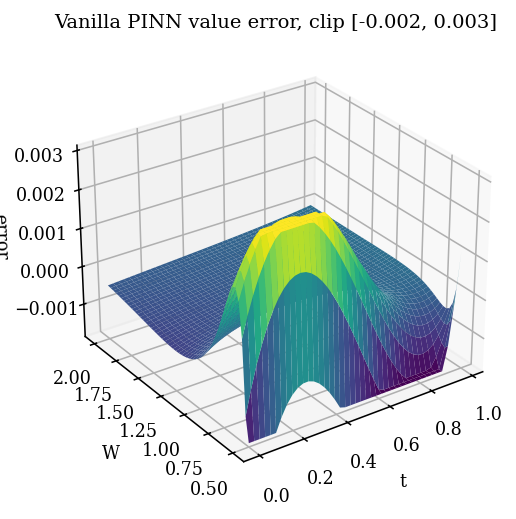
\includegraphics[width=0.72\textwidth]{surface_pinn_error.png}
\caption{Seed-0 power-scaled value error against the closed form. The surface is clipped to the 2nd and 98th percentiles of the error, here $[-1.78\times 10^{-3},\, 3.03\times 10^{-3}]$.}
\label{fig:pinnerr}
\end{figure}

\begin{figure}[H]
\centering
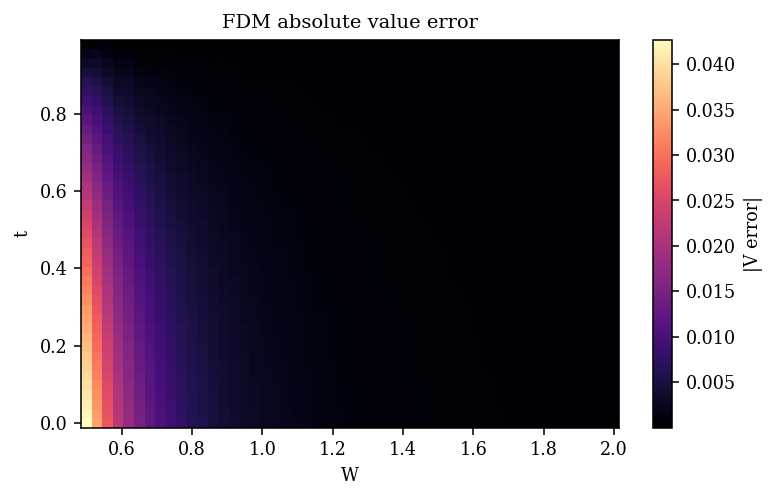
\includegraphics[width=0.46\textwidth]{error_heatmap_fdm.png}
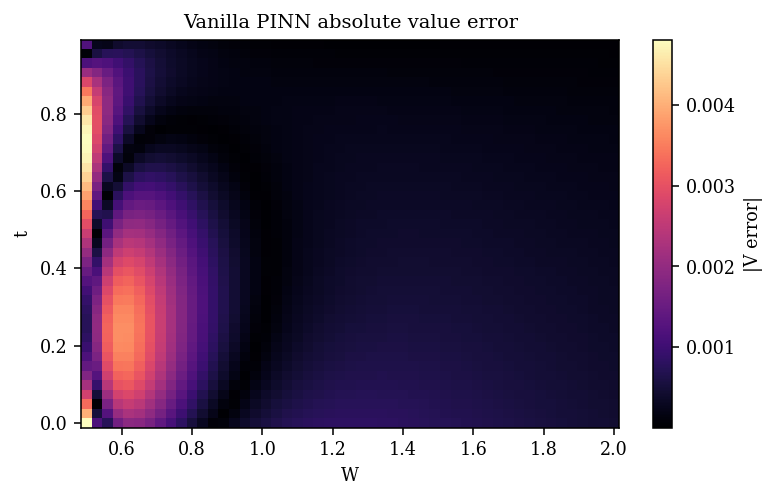
\includegraphics[width=0.46\textwidth]{error_heatmap_pinn.png}
\caption{Absolute value error of the E1 grid (left) and of the seed-0 power-scaled network (right). The color scales are separate. The network's value error is smaller than the grid's on this window.}
\label{fig:heat}
\end{figure}

\begin{figure}[H]
\centering
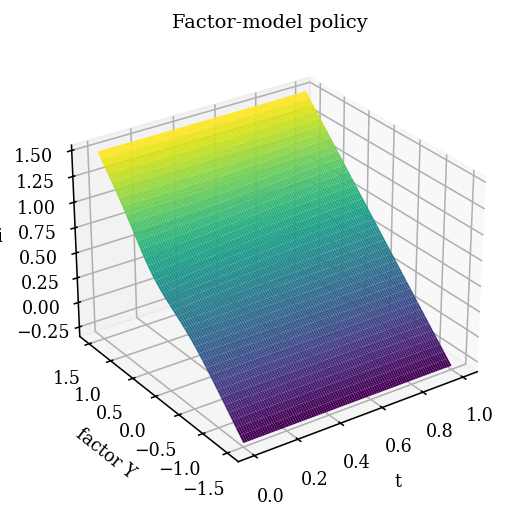
\includegraphics[width=0.72\textwidth]{surface_factor_policy.png}
\caption{E7 factor-grid policy over $(t,Y)$. At $Y=0$ the weight is about $0.50$, not the constant-opportunity value $0.60$.}
\label{fig:factor}
\end{figure}

\section{Reproducibility}
\label{sec:repro}

Work in \texttt{merton\_comparative\_study}. Check the drift identity with \texttt{python -m src.experiment.v2.check\_market}. Run one experiment with \texttt{python run\_one.py --exp E1}, and the same form through \texttt{E10}. Rebuild figures, without training, with \texttt{python -m src.experiment.v2.make\_figures}. Build this PDF with \texttt{pdflatex}, \texttt{bibtex}, and two further \texttt{pdflatex} passes. E1 aborts if the policy MAE exceeds $2\times 10^{-3}$ or the gap in $V(0,1)$ exceeds $5\times 10^{-3}$. Standard deviations for \Cref{tab:main1d} are in \texttt{results/v2/figures/table\_main.csv}: power-scaled policy $5.79\times 10^{-4}$, deep BSDE policy $7.20\times 10^{-3}$.

\section{Limits}
\label{sec:limits}

The rate $r$ is not estimated from prices. One equity and a one-factor opportunity set are not a large-$d$ test. The CRRA ansatz cannot be used as evidence that a value network has learned the weight. The deep BSDE is trained on $64$ time steps and scored on $252$-step wealth paths, so a gap between $Y_0$ and traded utility is expected. The constrained problem has an explicit projection at constant coefficients; the grid is reported because that is the reference a later non-explicit constraint would use, and because the network is not handed $\pi^{\star}$.

\bibliographystyle{plainnat}
\bibliography{refs_gbm}

\end{document}
